%! TeX program = lualatex

\RequirePackage{pdfmanagement-testphase}
\DocumentMetadata{
  pdfversion=2.0,
  % testphase=phase-III,        % автоматическое тегирование секций, параграфов и т.д.
  lang=ru
}
\documentclass[code]{wordcore}
% \documentclass{article}

\usepackage{fontspec}

\setmainfont{Times New Roman}[
  Path = ./font-times-new-roman/, % указывает текущую директорию
  UprightFont = *,
  ItalicFont = * - Italic,
  BoldFont = * - Bold,
  BoldItalicFont = * - Bold Italic
]

\setmonofont{consolas}[
  Path = ./consolas/, % указывает текущую директорию
  UprightFont = *,
  BoldFont = *-bold,
  ItalicFont = *-bold,
  BoldItalicFont = *-bold,
  % Scale=0.65,
]

% \setmonofont{Ubuntu mono}

\fancypagestyle{custom}{%
    \fancyhf{}% clears the footer and header
    % Header:
    \fancyhead[L]{}
    \fancyhead[C]{}
    \fancyhead[R]{}
    % Footer:
    \fancyfoot[L]{}
    \fancyfoot[C]{\thepage}
    \fancyfoot[R]{}
        % Tips:
        % ----
        % L: left, C: center, R: right
        % O: odd pages, E: even pages
        % ----
        % Example: \fancyghead[LO,RE]{Text}
        % will produce "Text" left in the header
        % on odd pages and right in the header on even pages.
    % Rules/ lines:
    \renewcommand{\headrulewidth}{0.0pt}
    \renewcommand{\footrulewidth}{0.0pt}
}
% Changing the pagestyle:
\pagestyle{custom}

\renewcommand{\cftsecnumwidth}{5.0em}

\begin{document}

\stepcounter{page}

\ttableofcontents

\newpage

\bbodysection{ВВЕДЕНИЕ}

Развитие цифровых технологий анализа микроструктур материалов и необходимость утилизации промышленных отходов способствуют активному внедрению интеллектуальных методов в материаловедении. Особенно актуально применение таких подходов при исследовании керамических композиционных материалов, созданных на основе золошлаков и шлаков тепловых электростанций. Эти материалы обладают высокими теплоизоляционными свойствами, механической прочностью и экологичностью. Однако их сложная пористая микроструктура требует точных, масштабируемых и воспроизводимых методов анализа.

Изображения микроструктур получают с помощью оптической или электронной микроскопии. Их количественный морфологический анализ до сих пор часто выполняется вручную или с минимальной автоматизацией. Такой подход не только трудоемок, но и снижает воспроизводимость результатов из-за влияния субъективного фактора. Это также затрудняет промышленную интеграцию метода и проведение масштабных исследований.

Современные методы искусственного интеллекта, включая сверточные нейронные сети, могут значительно ускорить анализ микроструктурных изображений. Однако их применение затрудняется нехваткой размеченных данных. Для сегментации слипшихся пор и других сложных структур требуется обучение на больших и разнообразных наборах данных. Однако их ручное создание требует временных и ресурсных затрат.

Цель работы --- разработка программы для генерации синтетических наборов данных, предназначенных для обучения моделей сегментации пористых структур. Создание такого инструмента должно решить проблему нехватки данных и ускорить разработку и тестирование систем анализа изображений. Были поставлены следующие задачи:
\begin{itemize}
	\item Разработать алгоритм генерации изображений с различными типами пор.
	\item Реализовать настройку параметров генерации через конфигурационный файл в формате JSON.
	\item Интегрировать алгоритм водораздела для создания точных масок сегментации, разделяющих слабопересекающиеся поры.
	\item Обеспечить генерацию изображений как с контрастным черно-белым фоном, так и с фоном, имитирующим текстурные шумы.
\end{itemize}

\section{ТЕОРЕТИЧЕСКАЯ ЧАСТЬ}

Геополимерные и стеклокомпозитные материалы на основе топливных шлаков --- это перспективный класс пористых композитов. Их сложная микроструктура формируется в условиях высокотемпературного синтеза и создает большие трудности при автоматическом анализе. Вследствие этого к качеству данных для обучения моделей предъявляются высокие требования.

Можно выделить две особенности, которые влияют на требования к генерируемому датасету:

\begin{itemize}
	\item Разнообразие форм пор

	      Форма пор в реальных материалах варьируется от округлых до вытянутых. Часто встречаются поры, по форме напоминающие рисовые зерна или вытянутые капли. Такая морфологическая неоднородность требует максимального разнообразия обучающих данных. Это необходимо, чтобы модель могла корректно идентифицировать объекты независимо от их геометрии.

	\item Слипшиеся поры

	      Наиболее сложный для анализа случай --- это перекрывающиеся или <<слипшиеся>> поры. Такие скопления воспринимаются стандартными алгоритмами как одна крупная структура, хотя физически представляют собой несколько объектов. Поэтому нейросеть должна научиться не просто находить такие скопления, но и корректно разделять их на составляющие. Для этого необходимо обучение на примерах с различной степенью перекрытия.

\end{itemize}

Учитывая эти структурные сложности, для обучения эффективной модели сегментации необходима обучающая выборка, которая бы их в полной мере отражала. Это и обосновывает необходимость создания программы для генерации синтетических изображений с разными морфологическими характеристиками.

\subsection{Классификация пор}

Для генерации обучающих данных необходимо формализовать типы структур, встречающиеся в реальных материалах. По анализу микрофотографий можно классифицировать поры по их морфологии и степени взаимного расположения. В таблице~\ref{tab:pore_classification} приведены целевые морфологические характеристики, которым должны соответствовать генерируемые поры.

\begin{table}[H]
	\centering
	\caption{Классификация пор на основе морфологических параметров}
	\label{tab:pore_classification}
	\resizebox{0.65\textwidth}{!}{
		\begin{tabular}{lcc}
			\toprule
			\textbf{Класс}                                                                 & \textbf{Пример} & \textbf{Перекрытие, \%} \\
			\midrule
			\multicolumn{3}{l}{\textbf{Одиночные поры}}                                                                                \\
			\midrule
			Округлая пора                                                                  &
			\vspace{8pt}
			\raisebox{-.5\height}{
\includegraphics[width=1.5cm]{fig/normal_pore.png}}      &
			\vspace{8pt}
			---                                                                                                                        \\
			Вытянутая пора                                                                 &
			\raisebox{-.5\height}{
\includegraphics[width=2.0cm]{fig/high_w_pore.png}}      &
			---                                                                                                                        \\
			\multicolumn{3}{l}{\textbf{Перекрытые поры}}                                                                               \\
			\midrule
			Соприкасающиеся                                                                &
			\vspace{8pt}
			\raisebox{-.5\height}{
\includegraphics[width=3.0cm]{fig/double_low_pore.png}}  &
			\vspace{8pt}
			Не более 10\%                                                                                                              \\
			Слабо перекрытые                                                               &
			\vspace{8pt}
			\raisebox{-.5\height}{
\includegraphics[width=2.5cm]{fig/double_med_pore.png}}  &
			\vspace{8pt}
			От 10 до 30\%                                                                                                              \\
			Сильно перекрытые                                                              &
			\vspace{8pt}
			\raisebox{-.5\height}{
\includegraphics[width=2.5cm]{fig/double_high_pore.png}} &
			\vspace{8pt}
			От 30\% и более                                                                                                            \\
			\bottomrule
		\end{tabular}
	}
\end{table}

Наличие перекрывающихся пор представляет собой основную проблему для автоматизированных систем анализа. Когда несколько пор слипаются, стандартные алгоритмы сегментации воспринимают их как единую пору. Это приводит к грубым ошибкам в количественном анализе: занижается общее число пор и искажается статистика их распределения по размерам.

Отсюда следует, основное требование к разрабатываемой программе --- это способность генерировать все перечисленные классы пор. Также слипшиеся поры должны разделяться границей, даже если на сгенерированном изображении они выглядят как единое целое. Это позволит обучить нейронную сеть распознавать границы объектов, а не их слияния.

\section{ПРАКТИЧЕСКАЯ ЧАСТЬ}

\subsection{Архитектура приложения}

Программа спроектирована по модульному принципу. Управляющий модуль \texttt{main.py} служит точкой входа: он инициализирует загрузку конфигурации, запускает цикл генерации, вызывает методы обработки и сохранения, а также выводит информацию о прогрессе.

Гибкость системы обеспечивает внешний конфигурационный файл \texttt{config\-.json}. За его чтение и валидацию отвечает модуль \texttt{config\_loader.py}. Структура файла разделена на четыре логических блока:

\begin{itemize}
	\item \texttt{image\_settings}: глобальные параметры изображений (размеры, количество).
	\item \texttt{pore\_settings}: морфологические параметры для каждого класса пор.
	\item \texttt{noise\_settings}: настройки фонового шума (интенсивность, диапазон яркости).
	\item \texttt{output\_settings}: пути сохранения и префиксы имен файлов.
\end{itemize}

\begin{figure}[H]
	\centering
	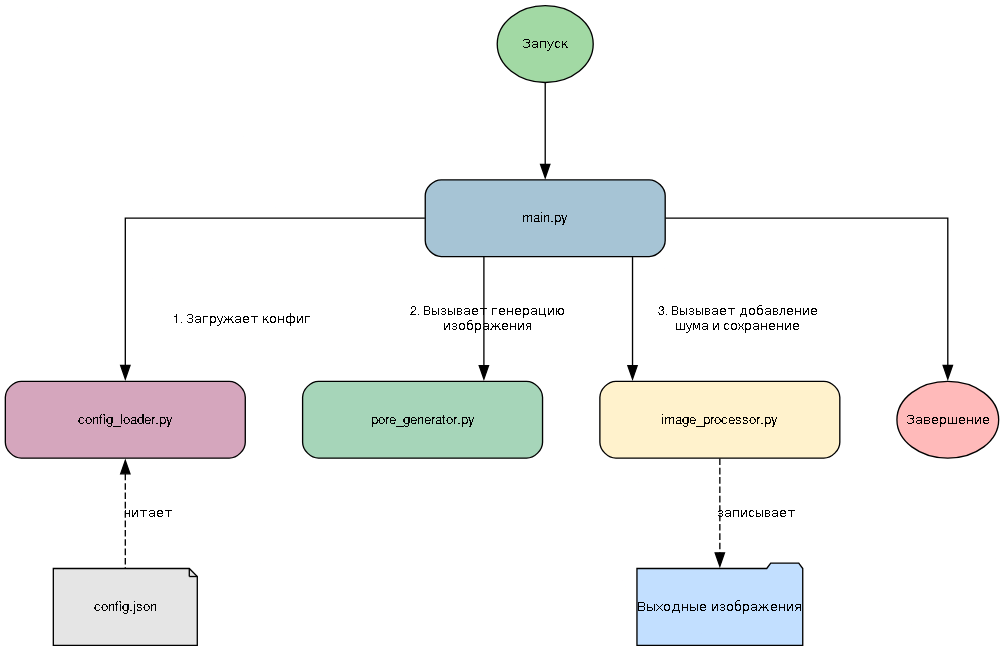
\includegraphics[width=1.0\textwidth]{fig/graphviz.png}
	\caption{Блок-схема работы приложения}
\end{figure}

Гибкость системы обеспечивает конфигурационный файл \texttt{config.json}, структура которого логически разделена на четыре основных блока:

\begin{itemize}
	\item Блок \texttt{image\_settings} определяет глобальные параметры датасета, такие как ширина, высота и общее количество изображений.
	\item В блоке pore\_settings задаются настройки для каждого класса пор: для одиночных \texttt{(single\_pores)}, слабо- и сильнопересекающихся \texttt{(weakly\_over\-lapping, strongly\_overlapping)}, а также дефектных \texttt{(defective\_pores)}.
	\item Параметры фонового шума, включая диапазон значений серого и интенсивность текстуры, контролируются в блоке \texttt{noise\_settings}.
	\item Блок \texttt{output\_settings} задает пути для сохранения данных и префикс для имен файлов.
\end{itemize}

\begin{code}
	\begin{minted}{json}
{
  "image_settings": {
    "width": 512,
    "height": 512,
    "total_images": 100
  },
  "pore_settings": {
    "single_pores": {
      "count_range": [5, 15],
      "radius_mean": 15,
      "radius_std": 3,
      "min_radius": 5,
      "max_radius": 30,
      "stretch_enabled": true,
      "stretch_factor_range": [1.0, 2.0],
      "rotation_enabled": true
    },
    "weakly_overlapping": {
      "count_range": [2, 5],
      "overlap_percentage_range": [0.1, 0.15],
      "radius_mean": 12,
      "radius_std": 2,
      "stretch_enabled": true,
      "stretch_factor_range": [1.0, 1.5],
      "rotation_enabled": true
    }
  },
  "noise_settings": {
    "min_gray_value": 200,
    "max_gray_value": 255,
    "noise_intensity": 0.1
  },
  "output_settings": {
    "clean_dir": "./output/clean_background",
    "noisy_dir": "./output/noisy_background",
    "file_prefix": "pore_image"
  }
}
  \end{minted}
\end{code}

\subsection{Алгоритм генерации пор}

Основная логика реализована в модуле \texttt{pore\_generator.py}. Процесс генерации построен последовательно: от простых изолированных объектов к сложным перекрывающимся структурам и последующей обработке.

\subsubsection{Генерация одиночных пор}

Начальный этап --- создание одиночных пор, реализованное в методе \texttt{\_add\_single\_pores}. Для придания реалистичности размер каждой поры генерируется на основе нормального распределения.

Для имитации вытянутых пор, которые часто встречаются в реальных материалах, программа позволяет выполнять эллиптическое растяжение. Метод \texttt{\_create\_elliptical\_pore} создает эллипс с заданным фактором растяжения и углом поворота. Перед размещением любой поры на основном изображении метод \texttt{\_is\_area\_free} проверяет, свободна ли целевая область, чтобы избежать неконтролируемых пересечений.

\begin{code}
	\begin{minted}{python}
# Метод для добавления одиночных пор на изображение
def _add_single_pores(self, image: np.ndarray, pore_info: Dict[str, List]) -> np.ndarray:
    # Загрузка настроек для одиночных пор из конфигурации
    settings = self.config['pore_settings']['single_pores']
    # Определение случайного количества пор для генерации в заданном диапазоне
    count = random.randint(*settings['count_range'])

    # Цикл генерации заданного количества пор
    for _ in range(count):
        # Генерация радиуса поры на основе нормального распределения
        radius = np.random.normal(settings['radius_mean'], settings['radius_std'])
        # Ограничение радиуса в заданных пределах (min/max)
        radius = int(np.clip(radius, settings['min_radius'], settings['max_radius']))

        # Инициализация параметров растяжения и угла поворота по умолчанию
        stretch_factor = 1.0
        angle = 0.0
        # Если растяжение включено в конфигурации
        if settings['stretch_enabled']:
            # Генерируется случайный фактор растяжения
            stretch_factor = random.uniform(*settings['stretch_factor_range'])
            # Если вращение включено, генерируется случайный угол
            if settings['rotation_enabled']:
                angle = random.uniform(0, 180)

        # Расчет эффективного радиуса для проверки столкновений и размещения
        effective_radius = int(radius * stretch_factor)
        # Если пора вытянутая (эллиптическая)
        if stretch_factor > 1.0:
            # Создание эллиптической поры на отдельном холсте
            pore_canvas, center = self._create_elliptical_pore(radius, stretch_factor, angle)
        else:
            # Создание обычной круглой поры
            canvas_size = radius * 2 + 1
            pore_canvas = np.ones((canvas_size, canvas_size), dtype=np.uint8) * 255
            cv2.circle(pore_canvas, (radius, radius), radius, 0, -1)
            center = radius

        # Попытка найти свободное место для размещения поры (до 100 попыток)
        placed = False
        for _ in range(100):
            # Генерация случайных координат центра поры
            x = random.randint(effective_radius, self.width - effective_radius)
            y = random.randint(effective_radius, self.height - effective_radius)

            # Проверка, свободна ли выбранная область
            if self._is_area_free(image, x, y, effective_radius):
                # Если область свободна, размещаем пору на основном изображении
                self._place_on_image(image, pore_canvas, center, x, y)
                # Сохранение информации о размещенной поре
                pore_info['single'].append({
                    'x': x, 'y': y, 'radius': radius,
                    'stretch_factor': stretch_factor, 'angle': angle
                })
                placed = True
                break  # Выход из цикла попыток, так как пора размещена
    return image

# Метод для создания эллиптической поры на временном холсте
def _create_elliptical_pore(self, radius: int, stretch_factor: float, angle: float) -> Tuple[np.ndarray, int]:
    # Создание временного холста, размер которого гарантирует, что эллипс поместится
    canvas_size = int(radius * 2 * stretch_factor * 1.5)
    canvas = np.ones((canvas_size, canvas_size), dtype=np.uint8) * 255
    center = canvas_size // 2

    # Определение осей эллипса
    axes = (int(radius * stretch_factor), radius)
    # Рисование черного эллипса на белом холсте
    cv2.ellipse(canvas, (center, center), axes, angle, 0, 360, 0, -1)

    return canvas, center

# Метод для проверки, свободна ли область на изображении
def _is_area_free(self, image: np.ndarray, x: int, y: int, radius: int, padding: int = 5) -> bool:
    # Определение границ проверяемой области с учетом отступов (padding)
    y_start = max(0, y - radius - padding)
    y_end = min(self.height, y + radius + padding)
    x_start = max(0, x - radius - padding)
    x_end = min(self.width, x + radius + padding)

    # Проверка, что все пиксели в области являются фоновыми (белыми, значение 255)
    return np.all(image[y_start:y_end, x_start:x_end] == 255)
  \end{minted}
\end{code}

\subsubsection{Создание перекрывающихся пор}

Логика, реализованная в методах \texttt{\_add\_weakly\_overlapping\_pores} и \texttt{\_add\-\_strongly\_overlapping\_pores}, основана на контролируемом размещении пор близко друг к другу. Сначала размещается первая пора, а позиция каждой следующей вычисляется относительно предыдущей.

Степень наложения контролируется параметром \texttt{overlap\_percentage\_range} из файла конфигурации. Расстояние между центрами двух пор (\(d\)) вычисляется по формуле: \( d = (r_1 + r_2) \times (1 - p) \), где \(r_1\) и \(r_2\)~--- радиусы пор, а \(p\)~--- процент пересечения. Таким образом, для слабо перекрытых пор расстояние будет больше, а для сильно перекрытых~--- меньше.

\begin{code}
	\begin{minted}{python}
# Получение случайного процента перекрытия из заданного в конфигурации диапазона
overlap_percent = random.uniform(*settings['overlap_percentage_range'])
# Координаты центра предыдущей поры, относительно которой размещается новая
prev_x, prev_y = centers[i-1]
# Эффективные радиусы предыдущей и текущей пор (с учетом растяжения)
effective_prev_radius = radii[i-1] * stretch_factors[i-1]
effective_radius = radius * stretch_factor

# Расчет расстояния между центрами пор на основе их радиусов и процента перекрытия
distance = (effective_prev_radius + effective_radius) * (1 - overlap_percent)
# Выбор случайного направления для размещения следующей поры
direction_angle = random.uniform(0, 2 * np.pi)

# Вычисление координат новой поры с использованием тригонометрии
x = int(prev_x + distance * np.cos(direction_angle))
y = int(prev_y + distance * np.sin(direction_angle))
  \end{minted}
\end{code}

\subsubsection{Разделение слипшихся пор}

Основнай задачей является корректное разделение соприкасающихся пор. Для этого применяется алгоритм водораздела, реализованный в методе \texttt{\_apply\-\_watershed}. Процесс состоит из нескольких шагов:

\begin{itemize}
	\item Инвертирование изображения: поры становятся белыми объектами на черном фоне.
	\item Построение карты расстояний: с помощью функции \texttt{scipy.ndimage.di\-stance\_transform\_edt} вычисляется расстояние от каждого пикселя поры до ближайшей границы. Геометрические центры пор становятся локальными максимумами на этой карте.
	\item Поиск маркеров: локальные максимумы определяются как маркеры, обозначающие центры отдельных пор.
	\item Применение алгоритма водораздела: алгоритм ''затапливает'' карту расстояний от маркеров, формируя границы там, где встречаются разные "бассейны".
\end{itemize}

\begin{code}
	\begin{minted}{python}
# Метод применяет алгоритм водораздела для разделения соприкасающихся объектов
def _apply_watershed(self, image: np.ndarray) -> np.ndarray:
    # Инвертирование изображения: поры становятся белыми, фон — черным
    inverted = cv2.bitwise_not(image)
    # Вычисление карты евклидовых расстояний от каждого пикселя объекта до фона
    distance = ndimage.distance_transform_edt(inverted)
    
    # Поиск локальных максимумов на карте расстояний — это будущие центры пор 
    coords = peak_local_max(distance, min_distance=3)
    # Создание маски, где отмечены только локальные максимумы
    local_maxima = np.zeros_like(distance, dtype=bool)
    local_maxima[tuple(coords.T)] = True
    
    # Создание карты маркеров, где каждая отдельная область  помечена уникальным целым числом
    markers = ndimage.label(local_maxima)[0]
    labels = watershed(-distance, markers, mask=inverted)
    
    # Создание нового изображения для отрисовки разделенных пор
    separated_image = np.ones_like(image) * 255
    # Отрисовка каждого сегмента на новом изображении
    for label in np.unique(labels):
        if label == 0:  # Пропуск фона
            continue
        separated_image[labels == label] = 0
        
    # Нахождение границ между сегментами с помощью детектора границ Canny
    edges = cv2.Canny(labels.astype(np.uint8), 1, 2)
    # Стирание границ, чтобы визуально разделить поры
    separated_image[edges > 0] = 255
    
    return separated_image
\end{minted}
\end{code}

\subsubsection{Имитация текстурного шума}

Для повышения устойчивости обучаемых нейросетевых моделей, программа генерирует для каждого набора пор две версии изображения: с контрастным фоном и с фоном, имитирующим текстурные шумы реальных микрофотографий. Этот функционал реализован в модуле \texttt{image\_processor}.

Интенсивность и диапазон яркости шума (например, от 200 до 255) настраиваются в блоке \texttt{noise\_settings} конфигурационного файла. Сгенерированный шумовой слой накладывается только на область фона, не затрагивая черные пиксели пор. В результате получается изображение, на котором поры четко выделяются на фоне реалистичной текстуры. Это позволяет обучать нейросеть быть менее чувствительной к вариациям фона.

\begin{code}
	\begin{minted}{python}
# Метод для генерации процедурного текстурного шума
def _generate_texture_noise(self, shape, intensity):
    height, width = shape
    # Инициализация пустого (черного) изображения для текстуры
    texture = np.zeros(shape)

    # Генерация и наложение нескольких слоев шума с разным масштабом и весом
    
    # 1. Низкочастотный шум
    scale1 = 50
    # Создается маленькое случайное изображение и растягивается до нужного размера с интерполяцией
    noise1 = cv2.resize(
        np.random.randn(height // scale1, width // scale1),
        (width, height),
        interpolation=cv2.INTER_CUBIC,
    )
    texture += noise1 * 0.5  # Добавление с весом 0.5

    # 2. Среднечастотный шум
    scale2 = 20
    noise2 = cv2.resize(
        np.random.randn(height // scale2, width // scale2),
        (width, height),
        interpolation=cv2.INTER_CUBIC,
    )
    texture += noise2 * 0.3  # Добавление с весом 0.3

    # 3. Высокочастотный шум
    scale3 = 5
    noise3 = cv2.resize(
        np.random.randn(height // scale3, width // scale3),
        (width, height),
        interpolation=cv2.INTER_CUBIC,
    )
    texture += noise3 * 0.2  # Добавление с весом 0.2

    # Нормализация полученной текстуры в диапазон [0, 1]
    texture = (texture - texture.min()) / (texture.max() - texture.min())
    # Получение диапазона яркости из настроек
    min_gray = self.noise_settings["min_gray_value"]
    max_gray = self.noise_settings["max_gray_value"]
    # Масштабирование текстуры до заданного диапазона яркости серого
    texture = texture * (max_gray - min_gray) + min_gray

    return texture
  \end{minted}
\end{code}

\subsection{Формирование выходных данных}

Для удобства дальнейшего использования в конвейерах машинного обучения программа создает структуру выходных файлов. Весь процесс управляется из главного модуля \texttt{main.py}. На основе путей, указанных в блоке \texttt{output\_settings} конфигурационного файла, создаются две директории: одна для изображений с чистым, контрастным фоном, а вторая для их аналогов с зашумленным фоном.

\begin{code}
	\begin{minted}{python}
# Функция для создания выходных директорий
def create_output_directories(config: Dict[str, Any]) -> None:
    # Создание директории для изображений с чистым фоном
    os.makedirs(config["output_settings"]["clean_dir"], exist_ok=True)
    # Создание директории для изображений с зашумленным фоном
    os.makedirs(config["output_settings"]["noisy_dir"], exist_ok=True)
    # Параметр exist_ok=True предотвращает ошибку, если директории уже существуют
  \end{minted}
\end{code}

\begin{figure}[H]
	\centering
	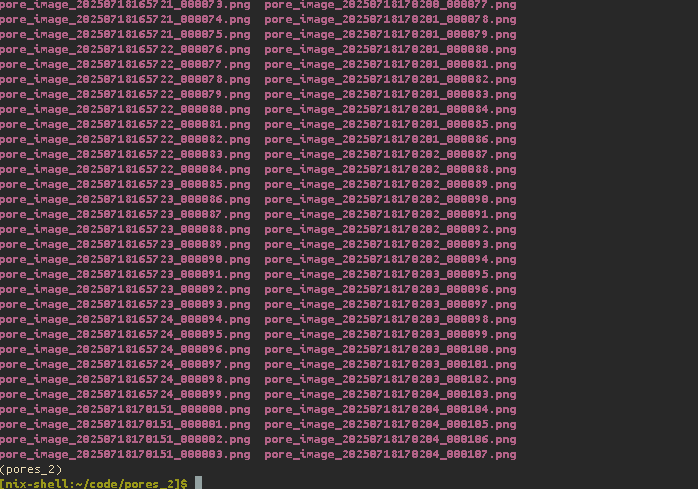
\includegraphics[width=0.75\textwidth]{fig/pores_output.png}
	\caption{Вывод сгенерированных изображений}
\end{figure}


\begin{figure}[H]
	\centering
	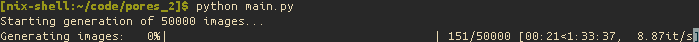
\includegraphics[width=0.75\textwidth]{fig/generate_pocessing.png}
	\caption{Процесс генерации}
\end{figure}

Для каждого сгенерированного набора пор создается пара изображений. Имена файлов генерируются уникальным образом с помощью функции \texttt{generate\-\_filename}, которая объединяет заданный префикс, временную метку (timestamp) для предотвращения перезаписи и порядковый номер. Пример имени файла: \texttt{pore\_image\_20231225153000\-\_000001.png}.

\section{РЕЗУЛЬТАТ РАБОТЫ ПРОГРАММЫ}

Ниже представлены примеры изображений, сгенерированных программой с использованием стандартной конфигурации. Для каждого типа структуры приводится пара изображений: слева — изображение с белым фоном, справа — его аналог с текстурированным.

\begin{figure}[H]
	\centering
	\begin{subfigure}[t]{0.48\textwidth}
		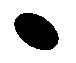
\includegraphics[width=\textwidth]{fig/signale_clean.png}
	\end{subfigure}
	\hfill % Небольшой отступ между картинками
	\begin{subfigure}[t]{0.48\textwidth}
		
\includegraphics[width=\textwidth]{fig/single_noisy.png}
	\end{subfigure}
	\caption{Пример генерации одиночной поры.}
\end{figure}

\begin{figure}[H]
	\centering
	\begin{subfigure}[t]{0.48\textwidth}
		
\includegraphics[width=\textwidth]{fig/low_verlap_noisy.png}
	\end{subfigure}
	\hfill
	\begin{subfigure}[t]{0.48\textwidth}
		
\includegraphics[width=\textwidth]{fig/low_overlap_noisy.png}
	\end{subfigure}
	\caption{Пример генерации слабопересекающихся пор.}
\end{figure}

\begin{figure}[H]
	\centering
	\begin{subfigure}[t]{0.48\textwidth}
		
\includegraphics[width=\textwidth]{fig/high_overlap_clean.png}
	\end{subfigure}
	\hfill
	\begin{subfigure}[t]{0.48\textwidth}
		
\includegraphics[width=\textwidth]{fig/high_overlap_noise.png}
	\end{subfigure}
	\caption{Пример генерации сильнопересекающихся пор, образующих сложные агломераты.}
\end{figure}

\begin{figure}[H]
	\centering
	\begin{subfigure}[t]{0.48\textwidth}
		
\includegraphics[width=\textwidth]{fig/defective_clean.png}
	\end{subfigure}
	\hfill
	\begin{subfigure}[t]{0.48\textwidth}
		
\includegraphics[width=\textwidth]{fig/defective_noisy.png}
	\end{subfigure}
	\caption{Пример генерации дефектных пор с неправильной формой}
\end{figure}


\begin{figure}[H]
	\centering
	\begin{subfigure}[t]{0.48\textwidth}
		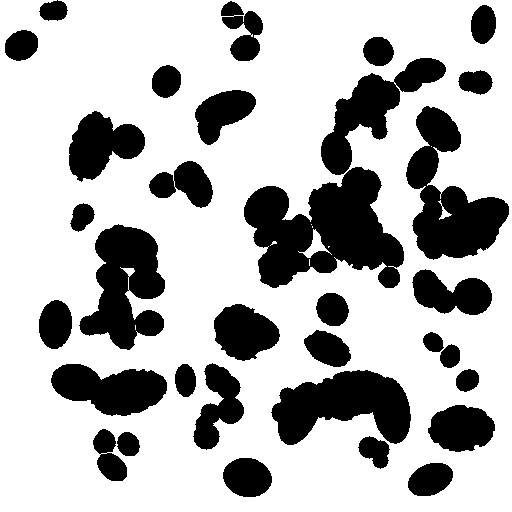
\includegraphics[width=\textwidth]{fig/full_clean.png}
	\end{subfigure}
	\hfill
	\begin{subfigure}[t]{0.48\textwidth}
		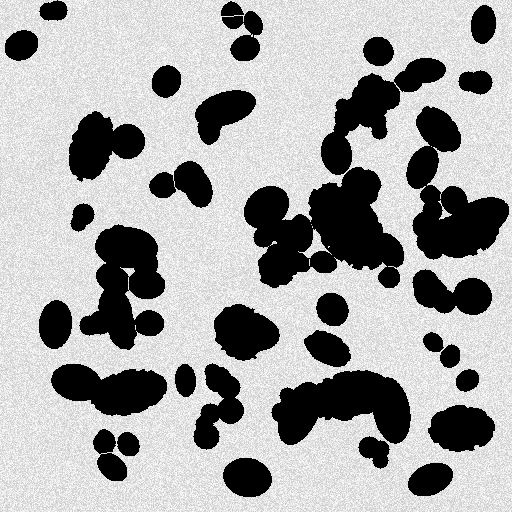
\includegraphics[width=\textwidth]{fig/full.png}
	\end{subfigure}
	\caption{Пример всего изображения}
\end{figure}

\newpage

\bbodysection{ЗАКЛЮЧЕНИЕ}

В ходе выполнения данного проекта были приобретены практические навыки в области процедурной генерации данных и разработки программного обеспечения на языке Python.

Работа над проектом была разделена на несколько этапов. Каждый этап был направлен на реализацию определенного функционала. Разработка базовых алгоритмов генерации позволила создавать изображения с порами различной морфологии: от одиночных округлых до вытянутых эллиптических. Реализация более сложных сценариев потребовала изучения и применения продвинутых алгоритмов, таких как метод водораздела для корректного разделения слабопересекающихся пор. Создание конфигурации через JSON-файл закрепило навыки проектирования масштабируемых и удобных для пользователя приложений.

Реализация программного комплекса потребовала активного применения библиотек компьютерного зрения (OpenCV, Scikit-image), инструментов для работы с многомерными массивами (NumPy), а также алгоритмов процедурной генерации.

Опыт, полученный в ходе этого проекта, служит важной основой для дальнейшего развития в области машинного обучения и анализа изображений. Созданный инструмент не только решает практическую задачу дефицита данных, но и демонстрирует умение применять теоретические знания для создания готовых программных продуктов.

\newpage
\nocite{*}
\pprintbibliography

\newpage



\begingroup

\singlespacing

\bbodysection{ПРИЛОЖЕНИЕ А}

\begingroup
\titleformat{\section}[block]
{\normalfont\normalsize\bfseries\centering}
{}{1em}{}

\section*{Листинг}

\endgroup

\textbf{main.py:}

\begin{code}
	\begin{minted}{python}
#!/usr/Bbin/env python3
"""
Main executable file for generating a dataset of pore images.
"""

import os
from datetime import datetime
from typing import Any, Dict

from tqdm import tqdm

from src.config_loader import ConfigLoader
from src.image_processor import ImageProcessor
from src.pore_generator import PoreGenerator


def create_output_directories(config: Dict[str, Any]) -> None:
    """Creates the output directories based on the configuration."""
    os.makedirs(config["output_settings"]["clean_dir"], exist_ok=True)
    os.makedirs(config["output_settings"]["noisy_dir"], exist_ok=True)


def generate_filename(config: Dict[str, Any], index: int) -> str:
    """Generates a unique filename using a timestamp and an index."""
    timestamp = datetime.now().strftime("%Y%m%d%H%M%S")
    prefix = config["output_settings"]["file_prefix"]
    return f"{prefix}_{timestamp}_{index:06d}.png"


def main() -> None:
    """Main function to run the image generation process."""
    config_loader = ConfigLoader("config.json")
    config = config_loader.load()

    create_output_directories(config)

    pore_generator = PoreGenerator(config)
    image_processor = ImageProcessor(config)

    total_images = config["image_settings"]["total_images"]
    print(f"Starting generation of {total_images} images...")

    for i in tqdm(range(total_images), desc="Generating images"):
        clean_image, pore_info = pore_generator.generate_image()

        noisy_image = image_processor.add_background_noise(clean_image)

        filename = generate_filename(config, i)

        clean_image_path = os.path.join(
            config["output_settings"]["clean_dir"], filename
        )
        noisy_image_path = os.path.join(
            config["output_settings"]["noisy_dir"], filename
        )

        image_processor.save_image(clean_image, clean_image_path)
        image_processor.save_image(noisy_image, noisy_image_path)

    print(f"\nGeneration complete! {total_images} images created.")
    print(f"Clean images saved to: {config['output_settings']['clean_dir']}")
    print(f"Noisy images saved to: {config['output_settings']['noisy_dir']}")


if __name__ == "__main__":
    main()
  \end{minted}
\end{code}

\textbf{config\_loader.py}

\begin{code}
	\begin{minted}{python}
"""
Module for loading and validating configuration.
"""

import json
import os
from typing import Any, Dict


class ConfigLoader:
    """Loads and validates configuration from a JSON file."""

    def __init__(self, config_path: str):
        self.config_path = config_path

    def load(self) -> Dict[str, Any]:
        """Loads the configuration from the JSON file."""
        if not os.path.exists(self.config_path):
            raise FileNotFoundError(f"Configuration file not found: {self.config_path}")

        with open(self.config_path, "r", encoding="utf-8") as f:
            config = json.load(f)

        self._validate_config(config)
        return config

    def _validate_config(self, config: Dict[str, Any]) -> None:
        """Validates the loaded configuration dictionary."""
        required_sections = [
            "image_settings",
            "pore_settings",
            "noise_settings",
            "output_settings",
        ]

        for section in required_sections:
            if section not in config:
                raise ValueError(f"Missing required section: {section}")

        image_settings = config["image_settings"]
        if image_settings["width"] <= 0 or image_settings["height"] <= 0:
            raise ValueError("Image dimensions (width, height) must be positive.")

        if image_settings["total_images"] <= 0:
            raise ValueError("Total images count must be positive.")
    
  \end{minted}
\end{code}

\textbf{image\_processor}

\begin{code}
	\begin{minted}{python}
"""
Module for image processing and saving operations.
"""

import random
from typing import Any, Dict, Tuple

import cv2
import numpy as np


class ImageProcessor:
    """Handles image manipulation tasks such as adding noise and saving."""

    def __init__(self, config: Dict[str, Any]):
        self.config = config
        self.noise_settings = config["noise_settings"]

    def add_background_noise(self, image: np.ndarray) -> np.ndarray:
        """Adds noise to the background (white pixels) of an image."""
        noisy_image = image.copy()
        background_mask = image == 255

        min_gray = self.noise_settings["min_gray_value"]
        max_gray = self.noise_settings["max_gray_value"]
        noise_intensity = self.noise_settings["noise_intensity"]

        random_noise_layer = np.random.randint(
            min_gray, max_gray + 1, size=image.shape, dtype=np.uint8
        )

        if noise_intensity > 0:
            texture_noise = self._generate_texture_noise(image.shape, noise_intensity)
            combined_noise_layer = (
                random_noise_layer * (1 - noise_intensity)
                + texture_noise * noise_intensity
            ).astype(np.uint8)
        else:
            combined_noise_layer = random_noise_layer

        noisy_image[background_mask] = combined_noise_layer[background_mask]

        return noisy_image

    def _generate_texture_noise(
        self, shape: Tuple[int, int], intensity: float
    ) -> np.ndarray:
        """Generates Perlin-like texture noise by combining multiple scales."""
        height, width = shape
        texture = np.zeros(shape, dtype=np.float32)

        scales = [50, 20, 5]  # Different scales for noise layers
        weights = [0.5, 0.3, 0.2]  # Weights for combining layers

        for scale, weight in zip(scales, weights):
            # Generate random noise and resize it to create a smoother effect
            random_field = np.random.randn(height // scale, width // scale)
            resized_noise = cv2.resize(
                random_field, (width, height), interpolation=cv2.INTER_CUBIC
            )
            texture += resized_noise * weight

        # Normalize texture to the desired gray value range
        min_gray = self.noise_settings["min_gray_value"]
        max_gray = self.noise_settings["max_gray_value"]

        # Prevent division by zero if texture is constant
        if texture.max() - texture.min() == 0:
            normalized_texture = np.full(
                shape, (min_gray + max_gray) / 2.0, dtype=np.float32
            )
        else:
            normalized_texture = (texture - texture.min()) / (
                texture.max() - texture.min()
            )
            normalized_texture = normalized_texture * (max_gray - min_gray) + min_gray

        return normalized_texture.astype(np.uint8)

    def save_image(self, image: np.ndarray, filepath: str) -> None:
        """Saves an image to the specified filepath."""
        cv2.imwrite(filepath, image)

    def apply_morphological_operations(self, image: np.ndarray) -> np.ndarray:
        """Applies morphological operations to improve image quality (e.g., smoothing edges)."""
        kernel_size = 3
        blurred = cv2.GaussianBlur(image, (kernel_size, kernel_size), 0.5)

        # Binary thresholding for sharp pore boundaries
        _, binary_image = cv2.threshold(blurred, 127, 255, cv2.THRESH_BINARY)

        return binary_image
  \end{minted}
\end{code}

\textbf{pore\_generator}

\begin{code}
	\begin{minted}{python}
"""
Module for generating various types of pores.
"""
import random
from typing import Any, Dict, List, Tuple

import cv2
import noise
import numpy as np
from scipy import ndimage
from skimage.feature import peak_local_max
from skimage.segmentation import watershed


class PoreGenerator:
    """Generates images with various types of simulated pores."""

    def __init__(self, config: Dict[str, Any]):
        self.config = config
        self.width = config['image_settings']['width']
        self.height = config['image_settings']['height']

    def generate_image(self) -> Tuple[np.ndarray, Dict[str, List]]:
        """Generates an image with all configured pore types."""
        image = np.ones((self.height, self.width), dtype=np.uint8) * 255
        pore_info = {
            'single': [],
            'weakly_overlapping': [],
            'strongly_overlapping': [],
            'defective': []
        }

        image = self._add_single_pores(image, pore_info)
        image = self._add_weakly_overlapping_pores(image, pore_info)
        image = self._add_strongly_overlapping_pores(image, pore_info)
        image = self._add_defective_pores(image, pore_info)

        return image, pore_info

    def _create_elliptical_pore(self, radius: int, stretch_factor: float, angle: float) -> Tuple[np.ndarray, int]:
        """Creates an elliptical pore on its own canvas."""
        canvas_size = int(radius * 2 * stretch_factor * 1.5)
        canvas = np.ones((canvas_size, canvas_size), dtype=np.uint8) * 255
        center = canvas_size // 2

        axes = (int(radius * stretch_factor), radius)
        cv2.ellipse(canvas, (center, center), axes, angle, 0, 360, 0, -1)

        return canvas, center

    def _place_on_image(self, image: np.ndarray, canvas: np.ndarray, canvas_center: int, x: int, y: int) -> np.ndarray:
        """Places a pore from its canvas onto the main image, handling boundaries."""
        pore_height, pore_width = canvas.shape

        y_start_img = max(0, y - canvas_center)
        y_end_img = min(self.height, y - canvas_center + pore_height)
        x_start_img = max(0, x - canvas_center)
        x_end_img = min(self.width, x - canvas_center + pore_width)

        y_start_pore = max(0, canvas_center - y)
        y_end_pore = y_start_pore + (y_end_img - y_start_img)
        x_start_pore = max(0, canvas_center - x)
        x_end_pore = x_start_pore + (x_end_img - x_start_img)

        img_slice = image[y_start_img:y_end_img, x_start_img:x_end_img]
        pore_slice = canvas[y_start_pore:y_end_pore, x_start_pore:x_end_pore]
        
        image[y_start_img:y_end_img, x_start_img:x_end_img] = np.minimum(img_slice, pore_slice)

        return image

    def _add_single_pores(self, image: np.ndarray, pore_info: Dict[str, List]) -> np.ndarray:
        """Adds single, non-overlapping pores to the image."""
        settings = self.config['pore_settings']['single_pores']
        count = random.randint(*settings['count_range'])

        for _ in range(count):
            radius = np.random.normal(settings['radius_mean'], settings['radius_std'])
            radius = int(np.clip(radius, settings['min_radius'], settings['max_radius']))

            stretch_factor = 1.0
            angle = 0.0
            if settings['stretch_enabled']:
                stretch_factor = random.uniform(*settings['stretch_factor_range'])
                if settings['rotation_enabled']:
                    angle = random.uniform(0, 180)

            effective_radius = int(radius * stretch_factor)
            if stretch_factor > 1.0:
                pore_canvas, center = self._create_elliptical_pore(radius, stretch_factor, angle)
            else:
                canvas_size = radius * 2 + 1
                pore_canvas = np.ones((canvas_size, canvas_size), dtype=np.uint8) * 255
                cv2.circle(pore_canvas, (radius, radius), radius, 0, -1)
                center = radius

            placed = False
            for _ in range(100):  # Max attempts
                x = random.randint(effective_radius, self.width - effective_radius)
                y = random.randint(effective_radius, self.height - effective_radius)

                if self._is_area_free(image, x, y, effective_radius):
                    self._place_on_image(image, pore_canvas, center, x, y)
                    pore_info['single'].append({
                        'x': x, 'y': y, 'radius': radius,
                        'stretch_factor': stretch_factor, 'angle': angle
                    })
                    placed = True
                    break
        return image

    def _add_weakly_overlapping_pores(self, image: np.ndarray, pore_info: Dict[str, List]) -> np.ndarray:
        """Adds groups of weakly overlapping pores, separated by the watershed algorithm."""
        settings = self.config['pore_settings']['weakly_overlapping']
        group_count = random.randint(*settings['count_range'])

        for _ in range(group_count):
            temp_image = np.ones((self.height, self.width), dtype=np.uint8) * 255
            pore_count = random.randint(2, 3)
            group_details = {'centers': [], 'radii': [], 'stretch_factors': [], 'angles': []}

            for i in range(pore_count):
                radius = int(np.clip(np.random.normal(settings['radius_mean'], settings['radius_std']), 5, 25))
                
                stretch_factor = 1.0
                angle = 0.0
                if settings['stretch_enabled']:
                    stretch_factor = random.uniform(*settings['stretch_factor_range'])
                    if settings['rotation_enabled']:
                        angle = random.uniform(0, 180)
                
                effective_radius = radius * stretch_factor
                margin = int(np.ceil(effective_radius))

                if i == 0:
                    x = random.randint(margin, self.width - margin)
                    y = random.randint(margin, self.height - margin)
                else:
                    overlap_percent = random.uniform(*settings['overlap_percentage_range'])
                    prev_x, prev_y = group_details['centers'][-1]
                    prev_radius = group_details['radii'][-1]
                    prev_stretch = group_details['stretch_factors'][-1]
                    
                    effective_prev_radius = prev_radius * prev_stretch
                    distance = (effective_prev_radius + effective_radius) * (1 - overlap_percent)
                    direction_angle = random.uniform(0, 2 * np.pi)
                    
                    x = int(prev_x + distance * np.cos(direction_angle))
                    y = int(prev_y + distance * np.sin(direction_angle))
                
                x = max(margin, min(x, self.width - margin))
                y = max(margin, min(y, self.height - margin))
                
                if stretch_factor > 1.0:
                    pore_canvas, center = self._create_elliptical_pore(radius, stretch_factor, angle)
                    self._place_on_image(temp_image, pore_canvas, center, x, y)
                else:
                    cv2.circle(temp_image, (x, y), radius, 0, -1)

                group_details['centers'].append((x, y))
                group_details['radii'].append(radius)
                group_details['stretch_factors'].append(stretch_factor)
                group_details['angles'].append(angle)

            separated_image = self._apply_watershed(temp_image)
            image = np.minimum(image, separated_image)
            pore_info['weakly_overlapping'].append(group_details)

        return image

    def _add_strongly_overlapping_pores(self, image: np.ndarray, pore_info: Dict[str, List]) -> np.ndarray:
        """Adds groups of strongly overlapping (merged) pores."""
        settings = self.config['pore_settings']['strongly_overlapping']
        group_count = random.randint(*settings['count_range'])
        
        for _ in range(group_count):
            pore_count = random.randint(2, 4)
            group_details = {'centers': [], 'radii': [], 'stretch_factors': [], 'angles': []}

            for i in range(pore_count):
                radius = int(np.clip(np.random.normal(settings['radius_mean'], settings['radius_std']), 5, 20))

                stretch_factor = 1.0
                angle = 0.0
                if settings.get('stretch_enabled', False):
                    stretch_factor = random.uniform(*settings['stretch_factor_range'])
                    if settings.get('rotation_enabled', False):
                        angle = random.uniform(0, 180)

                effective_radius = radius * stretch_factor
                margin = int(np.ceil(effective_radius))

                if i == 0:
                    x = random.randint(margin, self.width - margin)
                    y = random.randint(margin, self.height - margin)
                else:
                    overlap_percent = random.uniform(*settings['overlap_percentage_range'])
                    prev_x, prev_y = group_details['centers'][-1]
                    prev_radius = group_details['radii'][-1]
                    prev_stretch = group_details['stretch_factors'][-1]

                    effective_prev_radius = prev_radius * prev_stretch
                    distance = (effective_prev_radius + effective_radius) * (1 - overlap_percent)
                    direction_angle = random.uniform(0, 2 * np.pi)

                    x = int(prev_x + distance * np.cos(direction_angle))
                    y = int(prev_y + distance * np.sin(direction_angle))

                x = max(margin, min(x, self.width - margin))
                y = max(margin, min(y, self.height - margin))

                if stretch_factor > 1.0:
                    pore_canvas, center = self._create_elliptical_pore(radius, stretch_factor, angle)
                    self._place_on_image(image, pore_canvas, center, x, y)
                else:
                    cv2.circle(image, (x, y), radius, 0, -1)
                
                group_details['centers'].append((x, y))
                group_details['radii'].append(radius)
                group_details['stretch_factors'].append(stretch_factor)
                group_details['angles'].append(angle)

            pore_info['strongly_overlapping'].append(group_details)

        return image

    def _add_defective_pores(self, image: np.ndarray, pore_info: Dict[str, List]) -> np.ndarray:
        """Adds irregularly shaped defective pores."""
        settings = self.config['pore_settings']['defective_pores']
        count = random.randint(*settings['count_range'])

        for _ in range(count):
            radius = int(np.clip(np.random.normal(settings['radius_mean'], settings['radius_std']), 10, 30))
            
            stretch_factor = 1.0
            angle = 0.0
            if settings['stretch_enabled']:
                stretch_factor = random.uniform(*settings['stretch_factor_range'])
                if settings['rotation_enabled']:
                    angle = random.uniform(0, 180)

            x = random.randint(radius * 2, self.width - radius * 2)
            y = random.randint(radius * 2, self.height - radius * 2)

            defective_pore_canvas = self._create_defective_pore(
                radius, settings['deformation_factor'], stretch_factor, angle
            )
            
            pore_h, pore_w = defective_pore_canvas.shape
            center = max(pore_h, pore_w) // 2
            self._place_on_image(image, defective_pore_canvas, center, x, y)

            pore_info['defective'].append({
                'x': x, 'y': y, 'radius': radius,
                'stretch_factor': stretch_factor, 'angle': angle
            })

        return image

    def _is_area_free(self, image: np.ndarray, x: int, y: int, radius: int, padding: int = 5) -> bool:
        """Checks if a square area around a point is free (white)."""
        y_start = max(0, y - radius - padding)
        y_end = min(self.height, y + radius + padding)
        x_start = max(0, x - radius - padding)
        x_end = min(self.width, x + radius + padding)

        return np.all(image[y_start:y_end, x_start:x_end] == 255)

    def _apply_watershed(self, image: np.ndarray) -> np.ndarray:
        """Applies the watershed algorithm to separate touching objects."""
        inverted = cv2.bitwise_not(image)
        distance = ndimage.distance_transform_edt(inverted)
        
        coords = peak_local_max(distance, min_distance=3)
        local_maxima = np.zeros_like(distance, dtype=bool)
        local_maxima[tuple(coords.T)] = True
        
        markers = ndimage.label(local_maxima)[0]
        labels = watershed(-distance, markers, mask=inverted)
        
        separated_image = np.ones_like(image) * 255
        for label in np.unique(labels):
            if label == 0:
                continue
            separated_image[labels == label] = 0
            
        edges = cv2.Canny(labels.astype(np.uint8), 1, 2)
        separated_image[edges > 0] = 255
        
        return separated_image

    def _create_defective_pore(self, radius: int, deformation: float, stretch: float, angle: float) -> np.ndarray:
        """Creates a single deformed pore using Perlin noise."""
        canvas_size = int(radius * 2 * stretch * 1.5)
        canvas = np.ones((canvas_size, canvas_size), dtype=np.uint8) * 255
        center = canvas_size // 2

        axes = (int(radius * stretch), radius)
        temp_ellipse = np.zeros((canvas_size, canvas_size), dtype=np.uint8)
        cv2.ellipse(temp_ellipse, (center, center), axes, angle, 0, 360, 255, -1)

        scale, octaves, persistence = 0.1, 2, 0.5
        angle_rad = np.radians(angle)
        cos_a, sin_a = np.cos(angle_rad), np.sin(angle_rad)

        for i in range(canvas_size):
            for j in range(canvas_size):
                if temp_ellipse[i, j] > 0:
                    noise_val = noise.pnoise2(i * scale, j * scale, octaves=octaves, persistence=persistence)
                    
                    dx, dy = j - center, i - center
                    x_rot = dx * cos_a + dy * sin_a
                    y_rot = -dx * sin_a + dy * cos_a
                    
                    safe_radius = max(radius, 1)
                    safe_stretch_radius = max(radius * stretch, 1)

                    norm_dist = np.sqrt((x_rot / safe_stretch_radius)**2 + (y_rot / safe_radius)**2)
                    
                    modified_boundary = 1.0 + noise_val * deformation
                    if norm_dist <= modified_boundary:
                        canvas[i, j] = 0

        coords = np.argwhere(canvas == 0)
        if coords.size > 0:
            y_min, x_min = coords.min(axis=0)
            y_max, x_max = coords.max(axis=0)
            cropped = canvas[y_min:y_max+1, x_min:x_max+1]
            return cropped
        
        return np.ones((1,1), dtype=np.uint8) * 255 # Return a blank pixel if empty
  \end{minted}
\end{code}

\endgroup

\end{document}
